% 2025_tianjin_q17_fig1: 正方体 ABCD-A1B1C1D1，E/F 为 A1D1/C1B1 中点，G 在 CC1 上 CG=3GC1
\usetikzlibrary{calc}
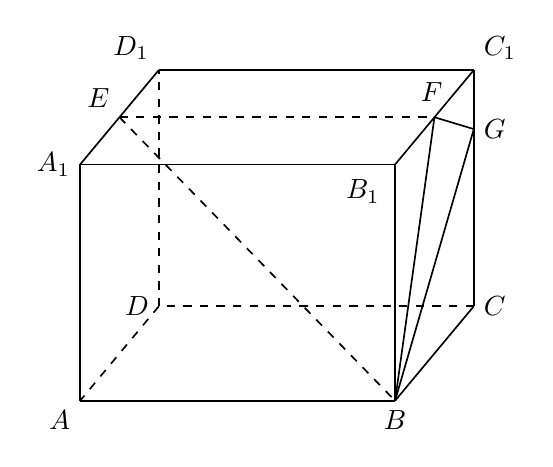
\begin{tikzpicture}[x=1cm,y=1cm,line width=.6pt]
  \coordinate (A) at (0,0);
  \coordinate (B) at (4,0);
  \coordinate (C) at (5,1.2);
  \coordinate (D) at (1,1.2);
  \coordinate (A1) at (0,3);
  \coordinate (B1) at (4,3);
  \coordinate (C1) at (5,4.2);
  \coordinate (D1) at (1,4.2);
  \coordinate (E) at (0.5,3.6);
  \coordinate (F) at (4.5,3.6);
  \coordinate (G) at (5,3.45);
  % 底面
  \draw (A) -- (B);
  \draw (B) -- (C);
  \draw[dashed] (C) -- (D);
  \draw[dashed] (D) -- (A);
  % 竖向棱
  \draw (A) -- (A1);
  \draw (B) -- (B1);
  \draw (C) -- (G);
  \draw (G) -- (C1);
  \draw[dashed] (D) -- (D1);
  % 顶面
  \draw (A1) -- (B1);
  \draw (B1) -- (C1);
  \draw (C1) -- (D1);
  \draw (D1) -- (A1);
  % 附加线段
  \draw[dashed] (E) -- (F);
  \draw[dashed] (E) -- (B);
  \draw (F) -- (B);
  \draw (F) -- (G);
  \draw (G) -- (B);
  % 标签
  \node[below left,font=\normalsize] at (A) {$A$};
  \node[below,font=\normalsize] at (B) {$B$};
  \node[right,font=\normalsize] at (C) {$C$};
  \node[left,font=\normalsize] at (D) {$D$};
  \node[left,font=\normalsize] at (A1) {$A_1$};
  \node[below left=2pt] at (B1) {$B_1$};
  \node[above right,font=\normalsize] at (C1) {$C_1$};
  \node[above left,font=\normalsize] at (D1) {$D_1$};
  \node[above left,font=\normalsize] at (E) {$E$};
  \node[above,font=\normalsize,xshift=-1.0pt,yshift=2pt] at (F) {$F$};
  \node[right,font=\normalsize] at (G) {$G$};
\end{tikzpicture}
